
\chapter{Testing of ARMAREST}

In our design and implementation, we assured that testing is simple and painless.
This is one of the reasons why our services in the \gls{backend} are split up into core and ice: 
It allows us to test the business logic in the core independently of the \gls{ice} connection.

\section{Test server}

Early on in the development, we realized that even though the \gls{frontend} could be developed on almost any device, 
testing it on the API required a connection to an \gls{armar} robot or simulation.
This prompted us to create the test server launcher as described in \nameref{design-changes}.
While implementing the test server, we wrote as little new code as we possibly could and re-used most of the existing \gls{backend} code.
Additionally, the new classes created for the test server were designed to be usable for unit testing as well.

The test server exposes the same API endpoints as the regular server and uses the regular service cores to do so.
However, it replaces the \gls{ice} connection with randomly generated data.
This allows \gls{frontend} developers to test their changes on the REST API even on devices without a connection to an \gls{armar} robot or simulation.

\section{Unit tests}

Most of the automated tests (unit, integration and end-to-end) that we planned will be written in the Quality Assurance phase.
However, we have already created multiple unit tests both in the \gls{backend} and in the \gls{frontend}:

\begin{description}
    \item[Backend: Logger] The logger contains two tests: The add\_message method of the core is tested through a unit test, and the entire service is tested with an integration test.
    \item[Backend: Kinematic] The kinematic\_unit contains two tests: One tests that the initial fetching of joints works, and the other one tests the update functions.
    \item[Frontend: RemoteGUI] The Remote GUI contains automated tests for the Label widget and the Button widget. Clicking the button should call a supplied function, which is tested as well.
\end{description}

\begin{figure}[h!]
    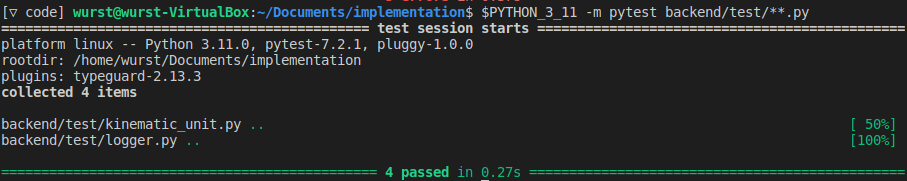
\includegraphics[width=0.8\linewidth]{images/pytest-result.png}
    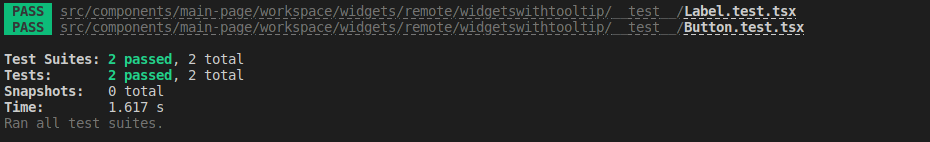
\includegraphics[width=0.8\linewidth]{images/jest-result.png}
\end{figure}
